\section{Capa de aplicación}
La capa de aplicación de CANae está dividida entre la denominada \textit{CANae Application Layer} y la \textit{CANae High Application Layer} Figura\ref{fig:CANAE}. La funcionalidad que brinda la capa de aplicación está dividad en diferentes elementos de servicios dentro del a capa de aplicación. Un elemento de servicios brinda un determinado servicio.

\begin{figure}[h!]
 \centering
 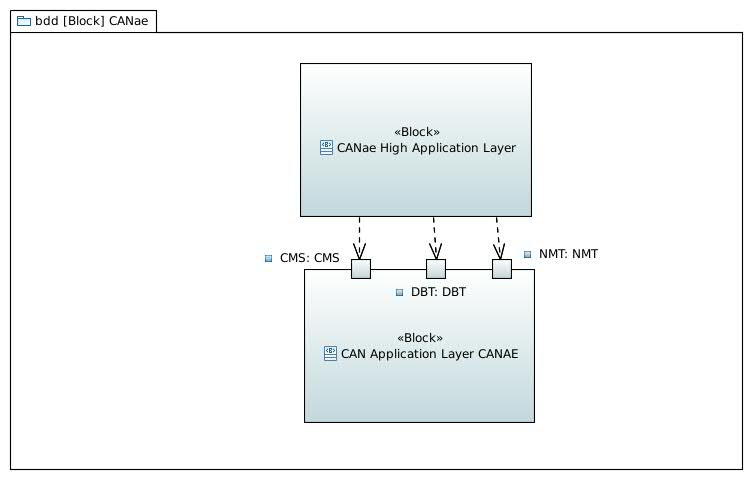
\includegraphics[scale=0.5]{images/Secciones/AppendixA/CANAE.JPG}
  \caption{Estructura de la capa de aplicación de CANae en alto nivel}
\label{fig:CANAE}
\end{figure}

Una capa de aplicación tiene las siguientes 4 funciones primitivas:
\begin{itemize}
\item Request: Una aplicación emite una petición a la capa de aplicación para solicitar un servicio.
  
\item Indication: Emitido por la capa de aplicación con destino una aplicación, para reportar de algún eveno interno detectado por la capa de aplicación, o indicar que un servicio fue solicitado.

\item Response: Emitido por la aplicación con destino la capa de aplicación para responder a una Indication previa.

\item Confirm: Emitido por la capa de aplicación para reportar el resultado de una peteción previa. 
\end{itemize}

\section{Tipos de servicios de la capa de aplicación}
Un tipo de servicio define las primitivas que intercambian las aplicaciones de usuario y los diferentes elementos de servicio que se encuentran dentro de la capa de aplicación. Los tipos de servicios posibles en CANae son los siguientes:
\begin{itemize}
\item Local serivice: Solo envuelve un elemento de servicio local. 

\item Confirmed service: Implica que uno o más elementos de servicio pares. La aplicación de usuario emite un request a su local service element. Este se transmite a sus elementos de servicios pares, la cual es enviada a la aplicación como una indicación. La otra aplicación emite un response que se transmite a la aplicación originante para confirmar la recepción del request. 

\item Provide initiated service: Implica solo el elemento de servicio local. El elemento de servicio detecta un evento no solicitado por la aplicación y emite una Indication. 
  
\end{itemize}

\section{CANae Application Layer}
En CANae se divide la tradicional capa de aplicación del modelo OSI en dos capas. En esta sección se estudia la \textit{CANae Application Layer}. Esta capa está conformada por 3 elementos de servicio:
\begin{itemize}
\item CAN based Message Specification (CMS): ofrece un ambiente orientado a objecto para diseñar aplicaciones de usuario. Esta entidad ofrece variables y eventos, y específica como un módulo pude acceder a las interfaces de CAN.
\item Network Managment (NMT): ofrece un ambiente orientado a objetos para permitir que un módulo (el NMT Master) se ocupe de la inicialización y posibles fallas  de otros módulos (NMT Slaves).
\item Distributor: ofrece el servicio para distribuir dinámicamente el identificador de para los diferentes nodos. 
\end{itemize}

Estos están basados en la capa de aplicación de CAN para la industria (CAN in Automation [CiA] International Users and Manufacturers Group e.V. CAN Application Layer for Industrial Applications). Estos elementos de servicios determinan el 'qué' puede hacer la capa. Estos son representados como interfaces(Figura \ref{fig:CANAE_APP_LAYER}).

\begin{figure}[h!]
 \centering
 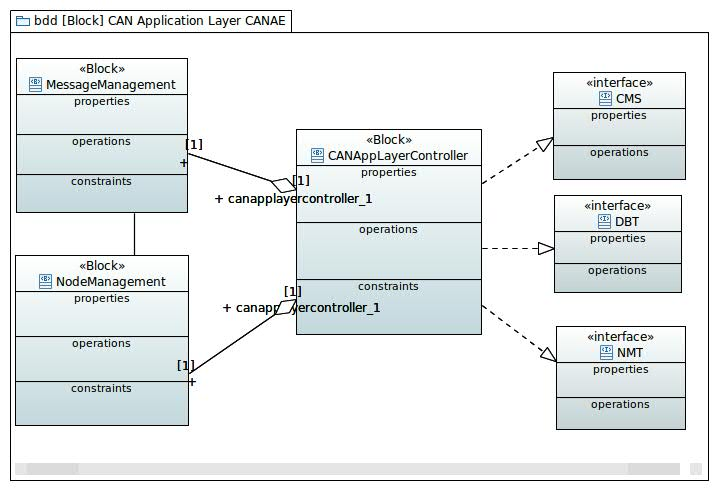
\includegraphics[scale=0.5]{images/Secciones/AppendixA/CAN_Application_Layer_CANAE.jpg}
  \caption{CANae Application Layer}
\label{fig:CANAE_APP_LAYER}
\end{figure}

Dentro de esta capa existen dos entidades importantes:
\begin{itemize}
\item Gestor de mensajes: este se encarga de gestionar los mensajes que son enviados y recibidos desde la red. Esta entidad debe ser capaz de determinar si el mensajes contiene datos o eventos. Trabaja en conjunto con el CMS.
  
\item Gestor de nodo: esta entidad se encarga de llevar el control de los nodos existenten en la red. En este nodo se encuentra la tabla de ruteo primario y secundario necesarios para la correcta comunicación.
  
\end{itemize}


